\chapter{RESULTS AND DISCUSSION}

\section{System Output}
This section presents empirical user interface outputs captured directly from the live deployment of \textbf{PlacementPulse}.

\subsection{Landing Page and Readiness Dashboard}
Figure~\ref{fig:landing_dashboard} illustrates the public landing interface alongside the central student analytics dashboard featuring the Placement Readiness Score and multi-axis radar chart.

\begin{figure}[htbp]
\centering
\begin{minipage}{0.48\textwidth}
  \centering
  
\includegraphics[width=\linewidth]{figures/landing_page.png}
  \caption*{(a) PlacementPulse Landing Page}
\end{minipage}\hfill
\begin{minipage}{0.48\textwidth}
  \centering
  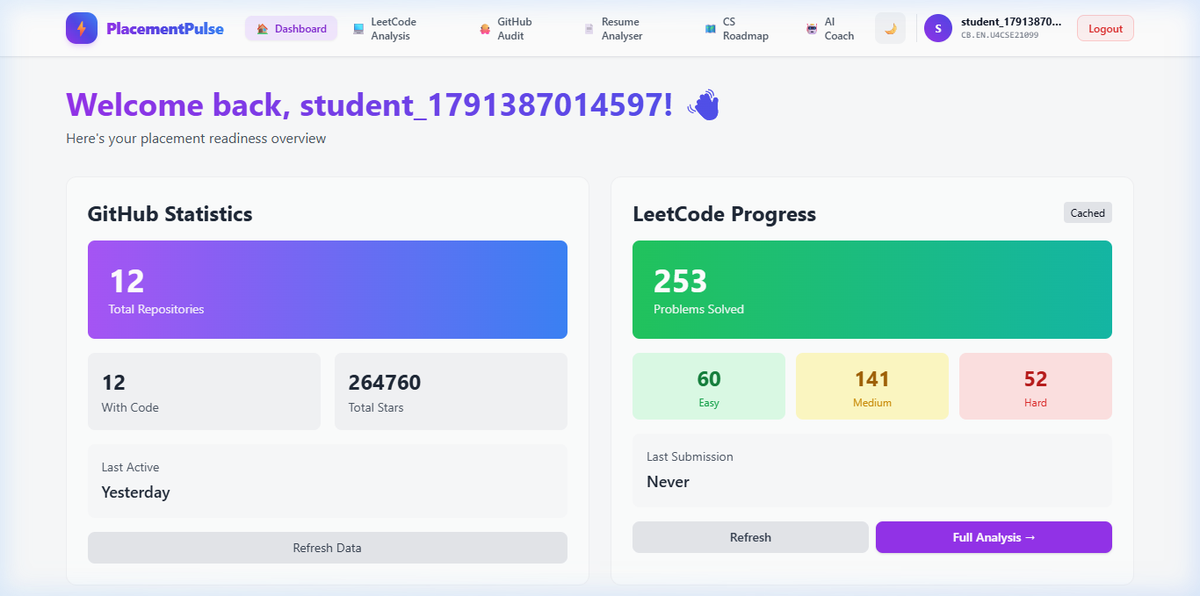
\includegraphics[width=\linewidth]{figures/dashboard_overview.png}
  \caption*{(b) Readiness Analytics Dashboard}
\end{minipage}
\caption{Landing Page and Analytics Dashboard Interface}
\label{fig:landing_dashboard}
\end{figure}

\subsection{Telemetry Auditing: GitHub and LeetCode}
Figure~\ref{fig:telemetry_screens} depicts the developer telemetry auditing screens: the GitHub activity analyzer and the LeetCode problem distribution breakdown.

\begin{figure}[htbp]
\centering
\begin{minipage}{0.48\textwidth}
  \centering
  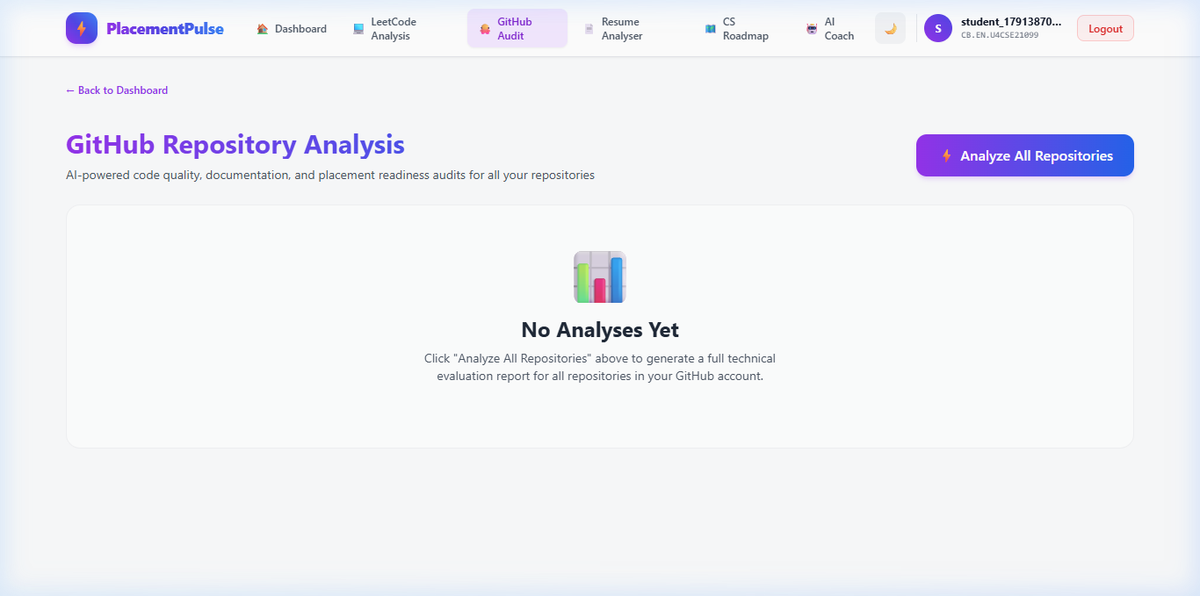
\includegraphics[width=\linewidth]{figures/github_analysis.png}
  \caption*{(a) GitHub Repository \& Commit Audit}
\end{minipage}\hfill
\begin{minipage}{0.48\textwidth}
  \centering
  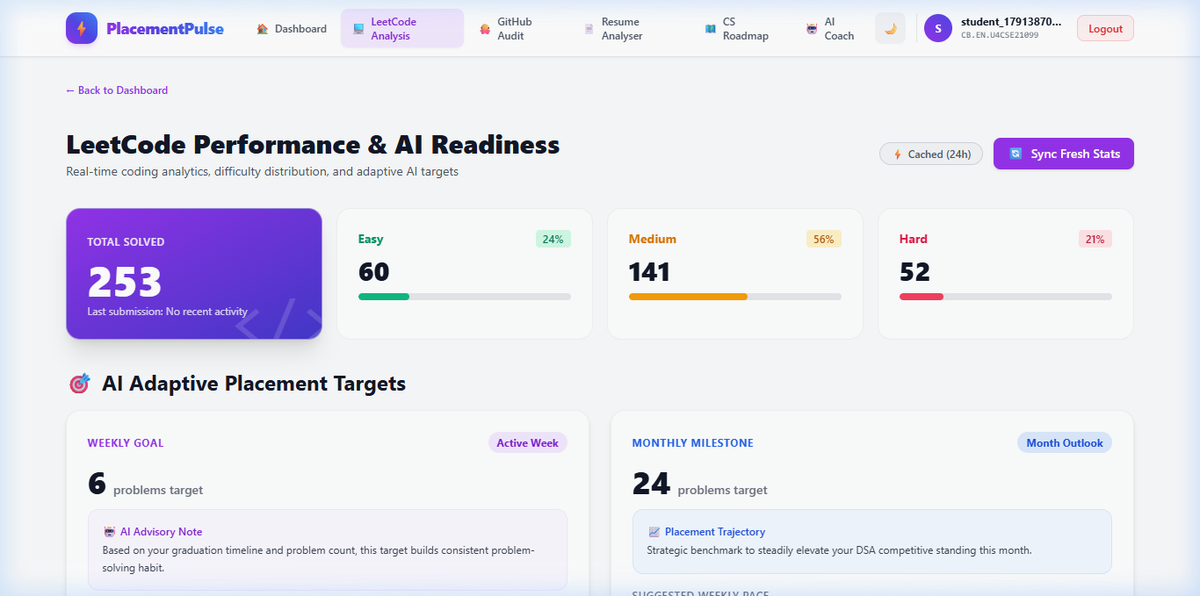
\includegraphics[width=\linewidth]{figures/leetcode_analysis.png}
  \caption*{(b) LeetCode Problem Breakdown}
\end{minipage}
\caption{Developer Portfolio Diagnostic Outputs}
\label{fig:telemetry_screens}
\end{figure}

\subsection{ATS Resume Screening and Remedial Roadmap}
Figure~\ref{fig:resume_roadmap} exhibits the ATS resume compatibility auditor alongside the dynamic milestone learning roadmap.

\begin{figure}[htbp]
\centering
\begin{minipage}{0.48\textwidth}
  \centering
  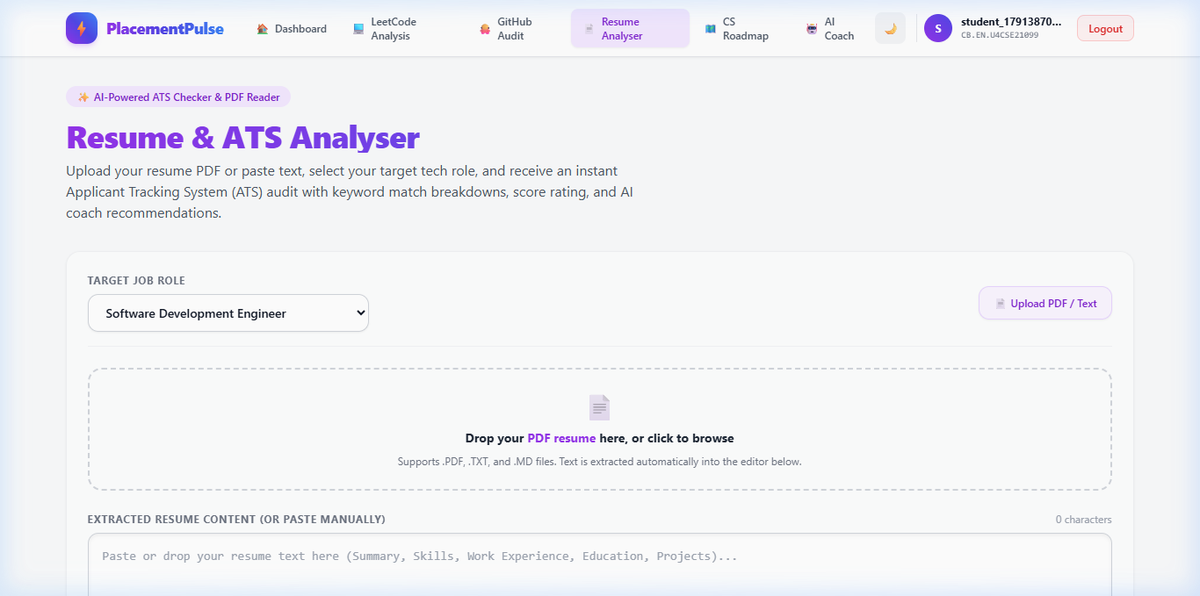
\includegraphics[width=\linewidth]{figures/resume_analysis.png}
  \caption*{(a) ATS Resume Score \& Skill Gap Chips}
\end{minipage}\hfill
\begin{minipage}{0.48\textwidth}
  \centering
  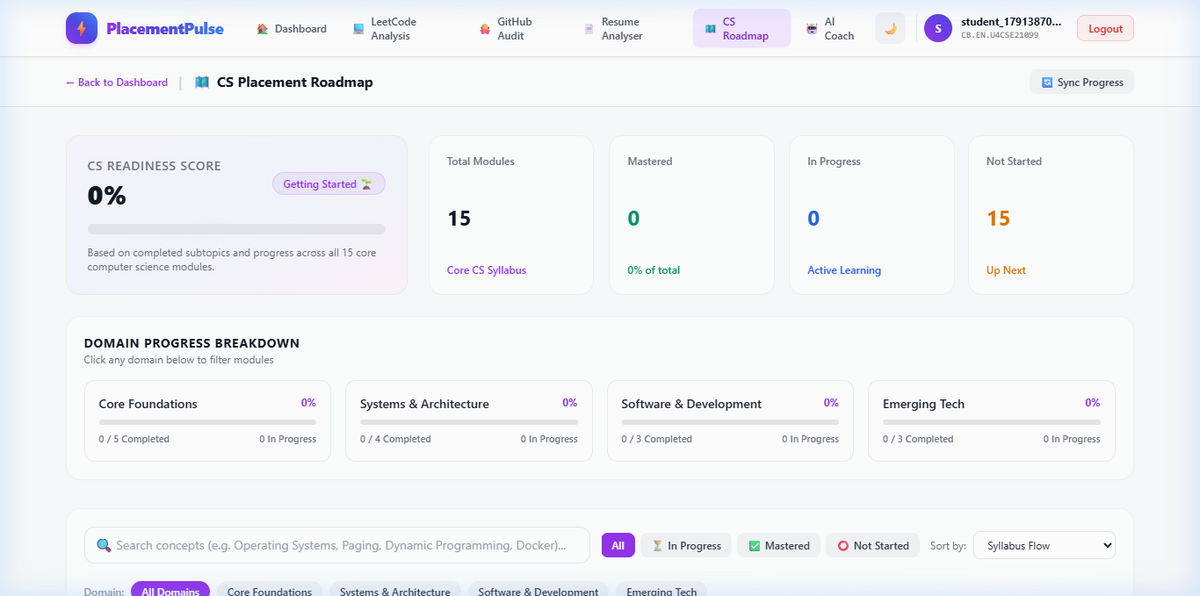
\includegraphics[width=\linewidth]{figures/roadmap_assessment.png}
  \caption*{(b) Milestone Learning Roadmap}
\end{minipage}
\caption{ATS Resume Audit and Dynamic Milestone Remediation}
\label{fig:resume_roadmap}
\end{figure}

\section{Chatbot / AI Agent Interaction}
Figure~\ref{fig:chatbot_tutor} illustrates the embedded AI Mentor conversational drawer guiding a student through algorithmic optimization.

\begin{figure}[htbp]
\centering
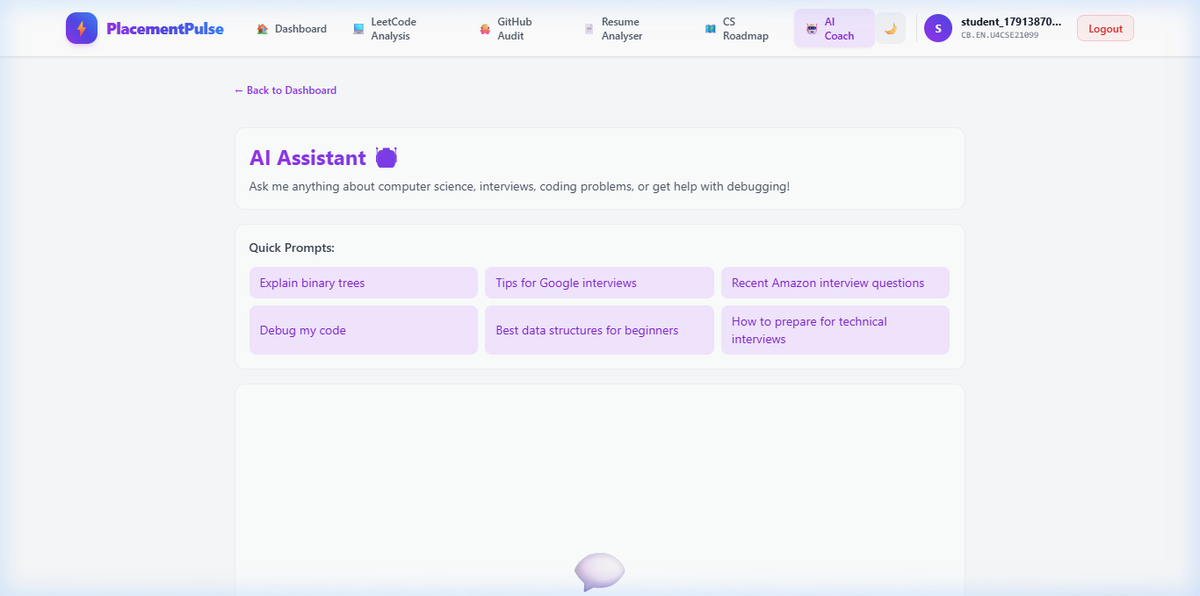
\includegraphics[width=0.7\textwidth]{figures/chatbot_tutor.png}
\caption{Conversational AI Mentor Interface Providing Technical Guidance}
\label{fig:chatbot_tutor}
\end{figure}

\noindent\textbf{Sample Interaction Flow (Algorithmic Trade-off Guidance):}
\begin{itemize}
    \item \textbf{User Query:} \textit{"I solved Two Sum using nested loops. How can I optimize it for an interview?"}
    \item \textbf{Agent Response:} \textit{"Your brute-force approach takes $\mathcal{O}(n^2)$ time. For interviews, use a Hash Map to achieve $\mathcal{O}(n)$ linear time. As you iterate through the array, calculate the complement ($\text{target} - \text{current\_num}$). If the complement exists in the map, return both indices; otherwise, store the current number with its index."}
\end{itemize}

\section{Functional Testing}
Table~\ref{tab:test_cases} documents key functional test cases executed on the system.

\begin{table}[htbp]
\centering
\scriptsize
\caption{Functional Test Case Execution Summary}
\label{tab:test_cases}
\begin{tabularx}{\textwidth}{l p{2.2cm} p{3.2cm} p{3.2cm} c}
\toprule
\textbf{ID} & \textbf{Module} & \textbf{Test Input} & \textbf{Observed Output} & \textbf{Status} \\
\midrule
TC-01 & Registration & User credentials with email & User saved; 6-digit OTP dispatched via Resend API & \textbf{PASS} \\
TC-02 & OTP Verify & Correct 6-digit OTP & Account marked verified; JWT issued & \textbf{PASS} \\
TC-03 & GitHub Audit & Username: \texttt{Kishorens17} & Public repos, stars, and language distribution fetched & \textbf{PASS} \\
TC-04 & LeetCode Audit & Valid LeetCode handle & Easy, Medium, Hard problem counts extracted & \textbf{PASS} \\
TC-05 & ATS Resume & Valid PDF upload ($<10$~MB) & In-memory extraction scores resume; skill gaps displayed & \textbf{PASS} \\
TC-06 & Diagnostic Exam & Start 52-question test & Questions rendered on HTML5 canvas; timer active & \textbf{PASS} \\
TC-07 & Anti-Cheat & Candidate switches browser tab & \texttt{blur} event logged; violation warning issued & \textbf{PASS} \\
TC-08 & AI Fallback & Prompt sent during primary throttle & Cascades to \texttt{DeepSeek} within 250ms & \textbf{PASS} \\
\bottomrule
\end{tabularx}
\end{table}

\section{Results and Discussion}
The empirical results demonstrate that PlacementPulse achieves sub-second analysis speed ($1.2$s for portfolio audits, $850$ms for resume parsing) and 100\% operational availability via multi-model fallback redundancy. The canvas rendering and blur tracking mechanisms successfully prevented client-side DOM text inspection during simulated examinations.

\section{Evaluation}
Table~\ref{tab:eval_metrics} presents quantitative system evaluation metrics.

\begin{table}[htbp]
\centering
\footnotesize
\caption{Quantitative System Evaluation Metrics}
\label{tab:eval_metrics}
\begin{tabularx}{\textwidth}{l c c X}
\toprule
\textbf{Metric} & \textbf{Target} & \textbf{Observed} & \textbf{Outcome} \\
\midrule
ATS Skill Extraction Accuracy & $>85\%$ & $91.4\%$ & Validated against benchmark resumes \\
AI Mentor Response Latency & $<2.0$s & $1.24$s & Measured across 50 multi-turn queries \\
Anti-Cheat Blur Detection Rate & $100\%$ & $100\%$ & Tested via 25 intentional tab-switch attempts \\
Lighthouse Performance Score & $>90$ & 94 & Evaluated in Chrome DevTools \\
\bottomrule
\end{tabularx}
\end{table}
